\usetikzlibrary{fit}

% keine Ahnung was das macht ;) ist vom indernet
% brauchts für den fitting node
\makeatletter
\tikzset{
  fitting node/.style={
    inner sep=0pt,
    fill=none,
    draw=none,
    reset transform,
    fit={(\pgf@pathminx,\pgf@pathminy) (\pgf@pathmaxx,\pgf@pathmaxy)}
  },  
  reset transform/.code={\pgftransformreset}
}
\makeatother

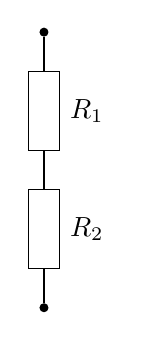
\begin{tikzpicture}[dot/.style={fill,circle,inner sep=1}]
  \def\rx {0.2}
  \def\ry {0.5}

  \node (dot) at (1,0) [draw,dot]{};
  
  \draw (1,-1) +(-\rx,-\ry) rectangle +(\rx,\ry) node[fitting node] (r1) {};

  \draw (1,-2.5) +(-\rx,-\ry) rectangle +(\rx,\ry) node[fitting node] (r2) {};

  \node (dot2) at (1,-3.5) [draw,dot]{};

  \draw (dot) -- (r1) -- (r2) -- (dot2) ;

  \node  [right] at (r1.east) {$R_1$};
  \node  [right] at (r2.east) {$R_2$};

\end{tikzpicture}
